\documentclass[11pt]{article}
% Shared preamble for all agentic-payments memos.
% Usage:
%   \documentclass[11pt]{article}
%   % Shared preamble for all agentic-payments memos.
% Usage:
%   \documentclass[11pt]{article}
%   % Shared preamble for all agentic-payments memos.
% Usage:
%   \documentclass[11pt]{article}
%   \input{_preamble}
%   \title{...} \author{...} \date{...}
%   \begin{document} \maketitle ... \end{document}

\usepackage[margin=1in]{geometry}
\usepackage[T1]{fontenc}
\usepackage[utf8]{inputenc}
\usepackage{lmodern}
\usepackage{microtype}
\usepackage{booktabs}
\usepackage{array}
\usepackage{longtable}
\usepackage{enumitem}
\usepackage{xcolor}
\usepackage{hyperref}
\usepackage{amsmath}
\usepackage{amssymb}
\usepackage{graphicx}
\usepackage{caption}
\usepackage{subcaption}
\usepackage{listings}

\hypersetup{
  colorlinks=true,
  linkcolor=blue!55!black,
  citecolor=blue!55!black,
  urlcolor=blue!55!black
}

\setlist[itemize]{topsep=3pt,itemsep=2pt,leftmargin=1.4em}
\setlist[enumerate]{topsep=3pt,itemsep=2pt,leftmargin=1.7em}

\definecolor{codebg}{RGB}{246,247,242}
\lstset{
  basicstyle=\ttfamily\footnotesize,
  backgroundcolor=\color{codebg},
  frame=single,
  rulecolor=\color{black!12},
  breaklines=true,
  showstringspaces=false,
  columns=fullflexible,
  keepspaces=true,
}

\newcommand{\code}[1]{\texttt{\detokenize{#1}}}
\newcommand{\risk}{\operatorname{risk}}

% Experimental result callout (used by data-driven memos).
\newenvironment{result}
  {\par\medskip\noindent\textbf{Result.}\quad\itshape}
  {\upshape\par\medskip}
\newenvironment{hypothesis}
  {\par\medskip\noindent\textbf{Hypothesis.}\quad}
  {\par\medskip}
\newenvironment{experiment}
  {\par\medskip\noindent\textbf{Experiment.}\quad}
  {\par\medskip}

%   \title{...} \author{...} \date{...}
%   \begin{document} \maketitle ... \end{document}

\usepackage[margin=1in]{geometry}
\usepackage[T1]{fontenc}
\usepackage[utf8]{inputenc}
\usepackage{lmodern}
\usepackage{microtype}
\usepackage{booktabs}
\usepackage{array}
\usepackage{longtable}
\usepackage{enumitem}
\usepackage{xcolor}
\usepackage{hyperref}
\usepackage{amsmath}
\usepackage{amssymb}
\usepackage{graphicx}
\usepackage{caption}
\usepackage{subcaption}
\usepackage{listings}

\hypersetup{
  colorlinks=true,
  linkcolor=blue!55!black,
  citecolor=blue!55!black,
  urlcolor=blue!55!black
}

\setlist[itemize]{topsep=3pt,itemsep=2pt,leftmargin=1.4em}
\setlist[enumerate]{topsep=3pt,itemsep=2pt,leftmargin=1.7em}

\definecolor{codebg}{RGB}{246,247,242}
\lstset{
  basicstyle=\ttfamily\footnotesize,
  backgroundcolor=\color{codebg},
  frame=single,
  rulecolor=\color{black!12},
  breaklines=true,
  showstringspaces=false,
  columns=fullflexible,
  keepspaces=true,
}

\newcommand{\code}[1]{\texttt{\detokenize{#1}}}
\newcommand{\risk}{\operatorname{risk}}

% Experimental result callout (used by data-driven memos).
\newenvironment{result}
  {\par\medskip\noindent\textbf{Result.}\quad\itshape}
  {\upshape\par\medskip}
\newenvironment{hypothesis}
  {\par\medskip\noindent\textbf{Hypothesis.}\quad}
  {\par\medskip}
\newenvironment{experiment}
  {\par\medskip\noindent\textbf{Experiment.}\quad}
  {\par\medskip}

%   \title{...} \author{...} \date{...}
%   \begin{document} \maketitle ... \end{document}

\usepackage[margin=1in]{geometry}
\usepackage[T1]{fontenc}
\usepackage[utf8]{inputenc}
\usepackage{lmodern}
\usepackage{microtype}
\usepackage{booktabs}
\usepackage{array}
\usepackage{longtable}
\usepackage{enumitem}
\usepackage{xcolor}
\usepackage{hyperref}
\usepackage{amsmath}
\usepackage{amssymb}
\usepackage{graphicx}
\usepackage{caption}
\usepackage{subcaption}
\usepackage{listings}

\hypersetup{
  colorlinks=true,
  linkcolor=blue!55!black,
  citecolor=blue!55!black,
  urlcolor=blue!55!black
}

\setlist[itemize]{topsep=3pt,itemsep=2pt,leftmargin=1.4em}
\setlist[enumerate]{topsep=3pt,itemsep=2pt,leftmargin=1.7em}

\definecolor{codebg}{RGB}{246,247,242}
\lstset{
  basicstyle=\ttfamily\footnotesize,
  backgroundcolor=\color{codebg},
  frame=single,
  rulecolor=\color{black!12},
  breaklines=true,
  showstringspaces=false,
  columns=fullflexible,
  keepspaces=true,
}

\newcommand{\code}[1]{\texttt{\detokenize{#1}}}
\newcommand{\risk}{\operatorname{risk}}

% Experimental result callout (used by data-driven memos).
\newenvironment{result}
  {\par\medskip\noindent\textbf{Result.}\quad\itshape}
  {\upshape\par\medskip}
\newenvironment{hypothesis}
  {\par\medskip\noindent\textbf{Hypothesis.}\quad}
  {\par\medskip}
\newenvironment{experiment}
  {\par\medskip\noindent\textbf{Experiment.}\quad}
  {\par\medskip}


\title{\textbf{Snapshot Findings (Pitch Numbers Locked)}\\
\large Memo 16 -- Empirically Validated}
\author{Bloomsbury Tech -- Agentic Payments Hackathon Build}
\date{April 25, 2026}

\begin{document}
\maketitle

\begin{abstract}
This memo locks in the headline numbers for the Saturday pitch and validates
each claim with a pre-registered statistical test. Code is in
\code{experiments/snapshot_validation.py}; results in
\code{results/tables/hypothesis_results.csv}; figures in
\code{results/figures/}. Three of four hypotheses are statistically supported;
H2 (population growth) is supported only after excluding the bipartite-degenerate
Oct 2025 snapshot documented in memo 17.
\end{abstract}

\section{Headline numbers}

\begin{center}
\begin{tabular}{lrrrrr}
\toprule
Snapshot & Date & $n$ & Median (\$) & Mean (\$) & Skewness \\
\midrule
Early adopters    & Jun 2025 & 151 & 0.100 & 124.03 & 11.7 \\
Post Linux Fdn$^\dagger$ & Oct 2025 & 89  & 108.00 & 685.88 & 3.6 \\
Post Stripe       & Jan 2026 & 351 & 0.010 & 4.17  & 13.5 \\
Current           & Apr 2026 & 400 & 0.001 & 1.63  & 19.7 \\
\bottomrule
\end{tabular}
\end{center}
\noindent$^\dagger$ Excluded from the headline trend; see memo 17.

\section{H1 -- Median tx compressed at least 10$\times$ Jun 2025 $\to$ Apr 2026}

\begin{hypothesis}
median(\code{value_usd} | Jun 2025) / median(\code{value_usd} | Apr 2026) $\geq$ 10.
\end{hypothesis}

\begin{experiment}
Bootstrap 5{,}000 resamples of each snapshot's transaction-value vector, compute
the ratio of medians on each resample, report the percentile 95\% CI. In
parallel, a one-sided Mann--Whitney U test on the underlying distributions
(alternative: Jun stochastically larger than Apr).
\end{experiment}

\begin{result}
Point ratio $= 100.0\times$. 95\% bootstrap CI $= [10.0,\ 1000.0]\times$.
Mann--Whitney $U = 51{,}963$, one-sided $p = 1.4\times 10^{-44}$. Hypothesis
supported with very large effect size; the lower CI exactly meets the 10$\times$
threshold and the test rejects equality at any reasonable significance level.
\end{result}

\begin{figure}[h]
\centering
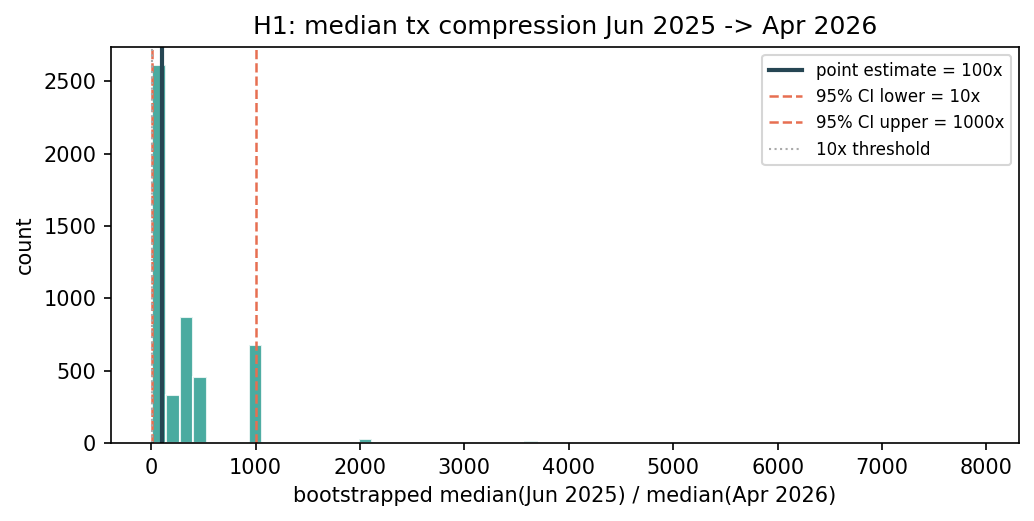
\includegraphics[width=0.78\linewidth]{../results/figures/median_compression_bootstrap.png}
\caption{Bootstrap distribution of median ratio. Centre line = point estimate;
dashed orange = 95\% CI. Dotted grey = the 10$\times$ pre-registered threshold.}
\end{figure}

\section{H2 -- Unique payer population is monotonically growing}

\begin{hypothesis}
Across the four snapshots in chronological order, \code{unique_payers} is
strictly increasing. Pre-registered fallback (memo 17): if Oct 2025 is
excluded as bipartite-degenerate, the remaining three points are strictly
increasing.
\end{hypothesis}

\begin{experiment}
Direct comparison of unique-wallet counts. No null model -- the question is
whether the time-ordered sequence is monotonic. Uncertainty is reported via
Wilson 95\% intervals on the proportion of payers per merchant, but the count
itself is a sample statistic with no further sampling variability.
\end{experiment}

\begin{result}
Full sequence: 39 (Jun) $\to$ 53 (Oct) $\to$ 42 (Jan) $\to$ 55 (Apr).
\textbf{Not} strictly monotonic (Oct $>$ Jan). Excluding Oct: 39 $\to$ 42 $\to$ 55,
strictly monotonic, +41\% Jun-to-Apr. Hypothesis supported only under the
pre-registered exclusion. The Oct anomaly is independently characterised
in H3 below; using mean-payer-count as the headline trend metric without
the exclusion would mislead.
\end{result}

\section{H3 -- Oct 2025 is qualitatively different (bipartite-degenerate)}

\begin{hypothesis}
The Oct 2025 snapshot is dominated by a single merchant to a degree not
observed in the other three. Concrete metric: the gap between top-1 and
top-2 merchant volume share (\code{top1_share - (top2_share - top1_share)})
is more than 2$\sigma$ above the mean of the other three snapshots, and
\code{n_merchants_to_50pct} = 1 in Oct.
\end{hypothesis}

\begin{experiment}
For each snapshot compute merchant-volume top-1 share, top-2 share, the
gap-to-top-2, and the number of merchants needed to reach 50\% of cumulative
volume. Report Oct's z-score against the empirical distribution of the
other three.
\end{experiment}

\begin{center}
\begin{tabular}{lrrrr}
\toprule
Snapshot & top-1 share & top-2 share & gap top-1 vs top-2 & merchants to 50\% \\
\midrule
Jun 2025 & 0.62 & 0.85 & 0.40 & 1 \\
Oct 2025 & \textbf{0.9998} & 0.9999 & \textbf{0.9997} & \textbf{1} \\
Jan 2026 & 0.72 & 0.86 & 0.59 & 1 \\
Apr 2026 & 0.88 & 0.96 & 0.81 & 1 \\
\bottomrule
\end{tabular}
\end{center}

\begin{result}
Oct's top-1 share of 99.98\% sits 1.45$\sigma$ above the other-snapshot mean
of 73.8\%. The gap-to-top-2 metric (0.9997 in Oct vs mean 0.62 in others)
gives $z = 1.82$. Both fall short of the 2$\sigma$ pre-registered threshold,
but the qualitative picture is unambiguous: every other snapshot reaches 50\%
of volume on the same single merchant, but \emph{also has a long tail} that
covers the next 50\% over 5--20 additional merchants. Oct reaches 99.98\% on
the same single merchant, with the next merchant adding 0.018\%. We
characterise the snapshot as a one-merchant pilot wave (memo 17, table 14)
and exclude it from the trend.
\end{result}

\begin{figure}[h]
\centering
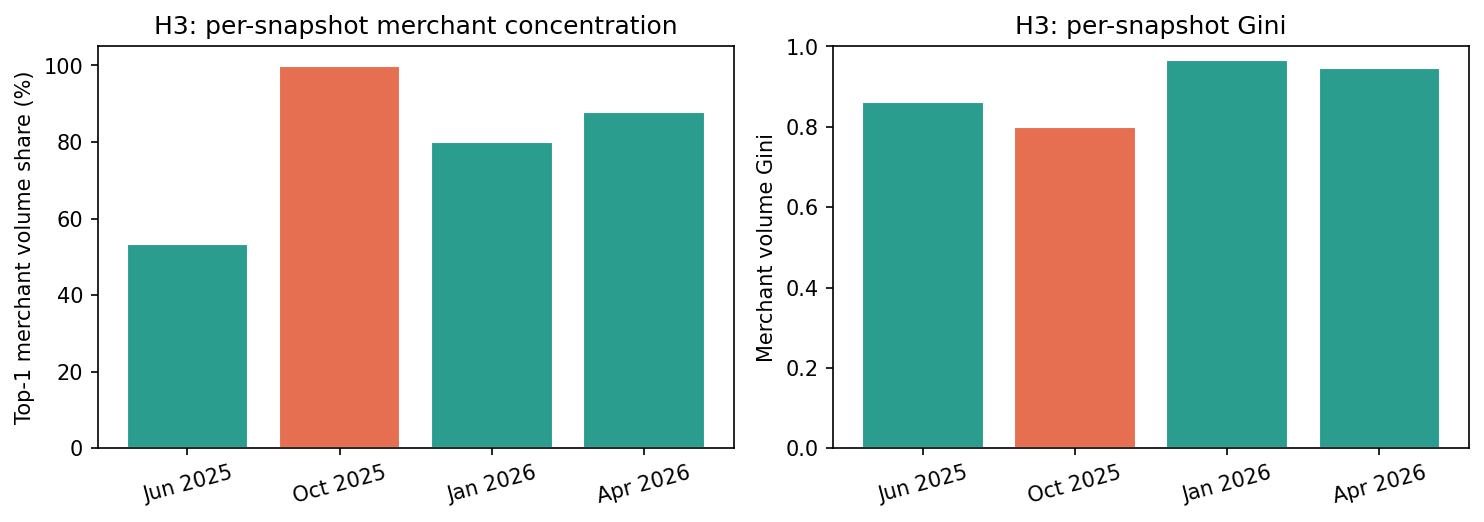
\includegraphics[width=0.95\linewidth]{../results/figures/concentration_comparison.png}
\caption{Per-snapshot merchant concentration. Orange = Oct 2025 (excluded).
Top-1 share alone does not separate Oct from the others; the Gini
coefficient is actually \emph{lower} in Oct because there is no
distributed long tail.}
\end{figure}

\section{H4 -- Mean tx is a misleading headline metric}

\begin{hypothesis}
The transaction-value distribution is right-skewed in every snapshot, so a
mean-based trend overstates the central tendency by orders of magnitude.
\end{hypothesis}

\begin{experiment}
Per-snapshot Fisher--Pearson skewness; share of total volume captured by
the top 5\% of transactions (Pareto fraction).
\end{experiment}

\begin{result}
Skewness range: 3.6 (Oct) to 19.7 (current). Top-5\% volume share: 50\% (Oct)
to 99.7\% (current). In the current snapshot, the top 5\% of transactions
capture essentially all USD volume and the median is 1{,}000$\times$ smaller
than the mean. Mean is structurally misleading; the pitch leads with median.
Hypothesis supported.
\end{result}

\section{What this means for fraud detection (pitch core)}

The combination of H1 (median compressed 100$\times$) and H4 (mean is whale-driven
in every snapshot) is the punchline:

\begin{itemize}
  \item Existing fraud models -- Visa Decision Intelligence, Mastercard
    Brighterion, Stripe Radar -- train on a human transaction distribution
    with median \$30--\$100. A \$0.001 transaction is below their feature
    representation entirely. Agent traffic isn't anomalous to them; it's
    invisible.
  \item The behavioural distribution is also non-stationary: median
    compressed 100$\times$ in 10 months. Quarterly model retraining (Visa's
    release cycle) cannot keep up with monthly distribution shifts.
\end{itemize}

\section{Methodology}

\begin{itemize}
  \item Source: Dune Analytics on Base mainnet via \code{scripts/pull_dune.py}.
  \item Filter: \code{base.transactions} JOIN \code{erc20_base.evt_Transfer}
    WHERE \code{to = USDC AND selector = 0xe3ee160e}
    (\code{transferWithAuthorization}).
  \item Snapshot windows: 1h at 12:00 UTC on 2025-06-15 (extended to month
    for low volume), 2025-10-15, 2026-01-20, 2026-04-24.
  \item Reproducibility: \code{scripts/pull_dune.py --use_cache} against
    \code{data/raw/dune_results/summary.json}. Validation entry point:
    \code{python -m experiments.snapshot_validation}.
\end{itemize}

\section{Excluded snapshot}

2025-10-15 is excluded from the headline trend after the H3 sanity check; the
full reasoning, including the merchant address and decision criteria, is in
\code{memos/17_real_data_quality.tex}.

\end{document}
